\section{Internet, IVV~NWZ, Computer\-Labs~\&~Co.}
\begin{multicols}{2}
	\fibelimgtext[below left]{
		\includegraphics[width=\columnwidth]{private/res/comics/hacker.pdf}
	}{Jan Tomaschoff\qquad© Cartoon-Caricature-Contors, Pfaffenhofen}
\subsection{WLAN für alle!}

Wo mittlerweile viele Restaurants und Cafés freien Internetzugang über WLAN zur Verfügung stellen und Parteien damit werben, das an Münsteraner Schulen fortzuführen, in einer Zeit, in der wissenschaftliches Arbeiten ohne den schnellen Austausch relativ großer Daten nicht mehr denkbar ist, gibt es natürlich auch an der Universität eures Vertrauens frei verfügbaren WLAN-Zugang für alle.
%Wenn sie an der \UniMuenster{}  arbeiten oder studieren oder einer am eduroam-Projekt teilnehmenden Hochschule sind.
Eine Anleitung zum Einrichten des WLANs findet sich für verschiedene Endgeräte in \cref{internet:wlan}.
Da für die Verbindung mit dem WLAN \enquote{uni-ms} ein Zertifikat nötig ist, bietet es sich an dieses zunächst über das offene Gäste-WLAN \enquote{GuestOnCampus} herunterzuladen.
Des Weiteren gibt es über das \enquote{eduroam}-Projekt auch die Möglichkeit das WLAN vieler Universitäten innerhalb und außerhalb Deutschlands zu nutzen.

Außerdem bekommt ihr noch ein ganzes Paket an Cloud-Speichern und könnt im Uni-Netz sogar von überall aus drucken oder eigentlich teure Bücher und Programme herunterladen.

\subsubsection{Und wie funktioniert das?}
Ihr erhaltet bereits mit eurer Einschreibung in die Uni eine Nutzerkennung, die aus eurem Vor- und Nachnamen gebildet wird, und ein dazugehöriges Passwort.
Zusätzlich erhaltet ihr eine Uni-E-Mail-Adresse -- hängt für diese einfach \texttt{@uni-muenster.de} an eure Nutzerkennung an.

Dadurch, dass ihr an der \UniMuenster{} Physik studiert, habt ihr einige praktische, kostenlose Angebote, die ihr mit eurer Nutzerkennung direkt nutzen könnt.

Technisch seid ihr dafür mit eurer Kennung Teil sogenannter Nutzergruppen, die euch verschiedene Berechtigungen geben. Für Studierende der Physik sind das zunächst ganz automatisch \texttt{u0dawin} (Studierende) und \texttt{p0stud} (Angehörige der Physik).

\subsection{Was kann man denn nun alles machen?}
So einiges. Der wichtigste Dienst ist dabei wohl euer E-Mail-Postfach.
Viele relevanten Infos werden euch darüber geschickt -- So zum Beispiel die Aufforderung, den Semesterbeitrag zu zahlen, oder die Information, dass eine Vorlesung kurzfristig ausfällt.
Ihr seid sogar verpflichtet, die Mails der Universität zu lesen -- Wenn ihr den Semesterbeitrag nicht zahlt, werdet ihr sogar exmatrikuliert -- also passt auf! 
Auch die Erinnerung zur Prüfungsanmeldung und unseren Newsletter sowie Infomails (mit denen wir uns aber sehr zurückhalten, wir wollen euch ja nicht "zuspammen", und auch wir kennen das Problem überfluteter Postfächer :) ) erhaltet ihr per Mail an eure Uni-Adresse.

Uns, die Fachschaft eures Vertrauens, erreicht ihr übrigens über die Adresse \email{fsphys@uni-muenster.de}.

\subsubsection{Portale}
Im Intranet (\url{https://www.uni-muenster.de/mystudy}) sind die wichtigsten Dienste der Uni zusammengefasst.
Dazu gehören insbesondere das E-Mail-Postfach, der Self-Service und das Vorlesungsverzeichnis (HIS~LSF) es gibt aber auch einen Kalender (der euch auch erinnert, wann ihr Bücher zurückgeben müsst) und von euch ausgewählte Newsfeeds\dots Wenn man das Intranet richtig nutzt, kann es sehr praktisch sein.

Auch sehr nützlich ist disco (\url{https://disco.uni-muenster.de}), das Suchsystem der ULB.
Hier sind der OPAC (ein Katalog- und Ausleihsystem der ULB) und viele weitere Verzeichnisse integriert, sodass ihr in vielen Millionen Dokumenten suchen könnt.
Ihr braucht also nicht jedes Mal zur ULB zu laufen, um Bücher zu verlängern.
Nochmal wichtiger sind Buch- und Literaturrecherchen, die ihr schnell und effektiv per Netz an den verschiedensten Stellen machen könnt.
Daneben gibt es über die ULB und den Fachbereich Physik auch einen kostenlosen Zugang zu allen wesentlichen wissenschaftlichen Zeitschriften und zu vielen Bücher z.\,B.\ von Springer.

Ruft dazu aus dem Uni-Netz (welches ihr auch von zu Hause aus über das sogenannte VPN der Uni erreicht) die Webseite \url{https://link.springer.com} auf und ladet das Buch eurer Wahl einfach herunter.

\begin{figure*}[t]
    \centering
    \fibelimgtext{
        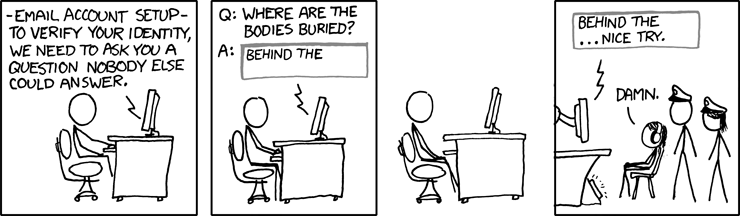
\includegraphics[width=\textwidth]{res/xkcd/565_security_question.png}
    }{\url{https://xkcd.com/565}}
\end{figure*}

%\begin{center}
%	\includegraphics[width=\columnwidth, height=0.3\textheight]{private/res/comics/computersuechtig.pdf}
%\end{center}

\subsubsection[Sichere Datencloud -- sciebo!]{Sichere Datencloud -- sciebo! \cref{internet:sciebo}}
Seit einigen Jahren bietet die \UniMuenster{} gemeinsam mit anderen nordrhein-westfälischen Hochschulen eine Dropbox-ähnliche Cloud an, die im Gegensatz zu anderen bekannten Online-Speicherdiensten betont nicht-kommerziell ist und viel Wert auf Datenschutz legt.
Ganz abgesehen davon, dass die Idee zur Cloud von einem Fachschaftler kam -- Danke, Markus :) -- ist Sciebo auch wegen seiner guten Umsetzung und einfacher Bedienoberfläche unbedingt empfehlenswert.
Einfach auf \url{https://www.sciebo.de} registrieren und dann mit \texttt{<nutzerkennung>@uni-muenster.de} als Benutzername und dem soeben gewählten Passwort anmelden.
Insgesamt bekommt man dort \SI{30}{\giga\byte} freien Speicherplatz, auf den man von überall aus über's Internet Zugriff hat.
Die automatische Synchronisation von Ordnern kann mit dem sciebo/ownCloud-Client eingerichtet werden.

\subsubsection{Zwei-Faktor-Authentifizierung}
Ein One Time Password (OTP) für die 2-Faktor-Authentifizierung braucht ihr hauptsächlich, um euch im IT-Portal oder im Self-Service anzumelden, aber auch für andere IT-Dienste der Uni Münster. Zu eurem Studienbeginn solltet ihr euch deshalb unbedingt darum kümmern, einen OTP-Generator einzurichten. Falls ihr dies, wie viele andere auch, vergesst, könnt ihr mit eurem Personalausweis zum CIT gehen, wo euch dann eins eingerichtet wird. 

\subsubsection{Mattermost}
Mattermost ist ein Chat-Service, um sich unter Personen an der Uni auszutauschen, ziemlich analog zu WhatsApp. Hier könnt ihr anderen Studierenden privat Nachrichten schreiben oder Gruppen für Gruppenarbeiten erstellen (auch wenn das nicht garantiert, dass euch jemand antwortet und euch nicht die ganze Arbeit alleine machen lässt). Das ganze funktioniert recht unkompliziert, da ihr einfach nach den Namen der Personen suchen könnt und nicht deren Telefonnummer oder Insta-Namen braucht. Oft erstellen auch die Dozierenden von Veranstaltungen ein Team für die Veranstaltung. Zu diesem Team gehören dann jeweils mehrere Kanäle, normalerweise einen für allgemeine Fragen, dem ihr automatisch beitretet, wenn ihr dem Team beitretet, und einzelne Kanäle für Übungsgruppen, zu denen euch dann eure Tutor*innen hinzufügen können. Diese Kanäle sind wie klassische Gruppen, die ihr von anderen Chat-Services kennt: Jeder kann Nachrichten schreiben und jeder kann die Nachrichten in der Gruppe lesen. Bei Kanälen für große Veranstaltungen ist wichtig, dass ihr diesen selbst beitreten müsst, oft über einen Link, den ihr im Learnweb findet. Eine genaue Anleitung dazu gibt es auf der Website der CIT~\cref{internet:cit_software}.

\subsubsection{Spielregeln}
Ihr habt einen ungefilterten, schnellen Zugang zum Internet und damit Zugriff auf alle möglichen Angebote.
Es sollte daher nicht unerwähnt bleiben, dass trotz der großen Zahl an Mitgliedern der Uni zurückverfolgt werden kann, wer Urheberrechtsverstöße und andere illegale Aktivitäten durchführt.
Ebenfalls führt z.\,B.\ der Versand von Spam und Viren zu einer Sperrung des Netzzugangs -- Die Sanktionen bei Zuwiderhandlung sind in der Benutzungsordnung geregelt.
Dies soll euch nicht abschrecken, dennoch solltet ihr die Spielregeln kennen.

\begin{center}
	\includegraphics[width=\columnwidth, height=0.3\textheight]{private/res/comics/computersuechtig.pdf}
\end{center}

\subsubsection{ComputerLabs \& Speicherplatz}
An quasi jedem Rechner der \UniMuenster{} habt ihr Zugriff auf euer persönliches Benutzerkonto -- Einfach Nutzerkennung und Passwort eingeben und los geht's.
Der Fachbereich Physik hat, auf mehrere Gebäude verteilt, "ComputerLabs" eingerichtet, an denen eine große Zahl an Rechnern für euch zur Verfügung stehen.
Mit eurer Nutzerkennung könnt ihr übrigens auch die Rechner in den Labs der Biologie und Chemie benutzen -- und umgekehrt.
Dass ihr überall dieselbe Arbeitsumgebung, euer Netzlaufwerk (Laufwerk \texttt{I:} mit \SI{10}{\giga\byte} Speicherplatz) und die gleichen Programme vorfindet, dafür ist gesorgt.
Außerdem gibt es noch allgemein zugängliche ComputerLabs wie die im CIT-Gebäude~'Einsteinstraße~60'.
Diese können von allen Angehörigen der Uni verwendet werden, allerdings stehen euch hier nicht dieselbe Software-Auswahl und Arbeitsumgebung zur Verfügung wie bei den Rechnern des naturwissenschaftlichen Zentrums (NWZ).
Standardmäßig ist beispielsweise nur euer CIT-Netzlaufwerk (Laufwerk \texttt{U:} mit \SI{4}{\giga\byte} Speicherplatz) und nicht das \texttt{I}-Laufwerk eingebunden.

Die Netzlaufwerke lassen sich auch von zu Hause aus via VPN erreichen, Anleitungen dazu gibt es auf den Webseiten von IVV NWZ und CIT.

Die ComputerLabs der Physik findet ihr an folgenden Orten:
\begin{description}
	\item[Angewandte Physik:] 10~Windows-PCs.
	\item[Lernzentrum:] 6~PCs
	\item[Institut~für~Kernphysik,] 2.~Stock: 11~Windows-PCs, Scanner, s/w-Laserdrucker.
	\item[Institut~für~Theoretische~Physik,] 4.~Stock: 9~Linux-PCs.
	\item[Institutsgruppe~1~(IG1):]~
		\begin{itemize}[leftmargin=1mm]
			% \item StudiBib, Erdgeschoss, Raum~13: Zwei Windows-PCs, Scanner, Farbdrucker.
			\item Institut für Technik und ihre Didaktik (Raum 220): 9~Windows-PCs, s/w-Laserdrucker.
			\item Physikalisches~Institut, 5.~Stock, Räume~504 und 520: insgesamt 9~Windows-PCs, A3-Flachbettscanner, s/w- und Farblaserdrucker.
			\item Institut~für~Festkörpertheorie, Raum~745 und 747: insgesamt 21~Windows-PCs, Scanner, s/w-Laserdrucker.
		\end{itemize}
	\item[Institut~für~Geophysik,] Corrensstr., Raum~301 und 333, je 10~Windows-PCs.
	\item[Seminar für Didaktik des Sachunterrichts]~\\(DDSU) im Leonardo-Campus~11, Raum~104: 9~Windows-PCs, s/w-Laserdrucker.
\end{description}

Die jeweiligen Kontaktadressen für Fragen und Probleme sind im jeweiligen ComputerLab bekannt gegeben.
Auf all diesen Computern ist ein sehr umfangreiches Software-Angebot installiert, sodass ihr dort direkt arbeiten könnt.
Eine Übersicht gibt es auf der Internetseite der IVV~NWZ~\cref{internet:ivvnwz}.

Der Begriff "IVV" stammt übrigens daher, dass es neben der CIT -- für die zentrale Bereitstellung von IT an der Uni zuständig -- an der Uni zehn sogenannte dezentrale "Informations-Verarbeitungs-Versorgungseinheiten" (IVV) gibt, die für bestimmte Bereiche zuständig sind.
Für die Fachbereiche Biologie, Chemie und Physik ist das die IVV~NWZ (IVV~4).

\subsubsection[Weitere Angebote der IVV~NWZ und der CIT]{Weitere Angebote der\\IVV~NWZ und der CIT}
Sowohl die IVV~NWZ (mit "nwzcitrix" via Uni-VPN) als auch die CIT (mit "rd.wwu.de") betreiben Remote-Desktop-Server, auf die ihr von Zuhause aus zugreifen könnt.
Damit habt ihr auch von Zuhause aus Zugriff auf die meiste Software und könnt damit arbeiten.
Das Stichwort "Cloud" fällt meist irgendwann in diesem Zusammenhang und sollte heutzutage jedem bekannt sein.
Etwas Ähnliches bieten IVV und CIT schon seit vielen Jahren allen Studierenden an.

Weitere Informationen hierzu und vielen weiteren Angeboten sowie Anleitungen gibt es bei der IVV~NWZ~\cref{internet:ivvnwz} und bei der CIT~\cref{internet:cit}, sowie in der Ersti-Woche und bei uns~\cref{internet:fsphys_software}.

\subsubsection{Software für Zuhause}
Für Studierende gibt es bei der CIT zwei interessante Softwarepakete, die insbesondere auch für den privaten Einsatz auf den eigenen Computern vorgesehen sind.
Interessant ist vor allem die Anti-Virus-Software (Sophos), welche von der Uni für alle bezahlt wird.
Zusätzlich können viele weitere Programme, die die CIT betreut, auch auf dem eigenen Rechner installiert und unter einigen Bedingungen genutzt werden~\cref{internet:cit_software}.

Die IVV~NWZ ermöglicht zudem allen zugehörigen Studierenden den Zugriff auf das "Azure Dev Tools for Teaching"-Programm von Microsoft.
Damit habt ihr Zugriff auf fast die gesamte Software-Palette von Microsoft, ausgeschlossen sind nur einige Office-Programme. 
Microsoft Office-Produkte bekommt ihr allerdings auch kostenlos, und zwar über "Lizenzen" im IT-Portal, siehe \cref{internet:cit}.
Diese Software dürft ihr ausdrücklich auch auf privaten Rechner installieren.
Weitere Programme wie die Mathematik-Software "Mathematica" (vielen vielleicht bereits durch die -- übrigens fürs Studium häufig nützliche -- Website WolframAlpha \cref{internet:wolfram_alpha} bekannt) können ebenfalls unter verschiedenen Bedingungen bezogen werden -- Mathematica kann beispielsweise nur im Uni-Netzwerk (d.\,h.\ zum Beispiel von Zuhause über eine VPN-Verbindung) genutzt werden.
Weitere Infos findet ihr wieder unter \cref{internet:ivvnwz}, \cref{internet:cit} und \cref{internet:fsphys_software}.

\subsection{Links}
\begin{flushleft}
	\begin{fibelurl}
		\url{https://www.uni-muenster.de/IT/services/kommunikation/wlan/}
		\label{internet:wlan}
	\end{fibelurl}
	\begin{fibelurl}
		\url{https://www.sciebo.de}
		\label{internet:sciebo}
	\end{fibelurl}
	\begin{fibelurl}
		\url{https://www.uni-muenster.de/NWZ}
		\label{internet:ivvnwz}
	\end{fibelurl}
	\begin{fibelurl}
		\url{https://www.uni-muenster.de/IT}
		\label{internet:cit}
	\end{fibelurl}
	\begin{fibelurl}
		\url{https://www.uni-muenster.de/Physik.FSPHYS/service/software}
		\label{internet:fsphys_software}
	\end{fibelurl}
	\begin{fibelurl}
		\url{https://www.uni-muenster.de/IT/Software/Uebersicht.html}
		\label{internet:cit_software}
	\end{fibelurl}
	\begin{fibelurl}
		\url{https://www.wolframalpha.com}
		\label{internet:wolfram_alpha}
	\end{fibelurl}
\end{flushleft}

\fibelsig{Simon, Benedikt, APN, Sarah}

\begin{center}
\fibelimgtext{
	\includegraphics[width=\columnwidth]{res/xkcd/722_computer_problems.png}
}{\url{https://xkcd.com/722}}
\end{center}

\end{multicols}

%\begin{center}
%\fibelimgtext{
	%\includegraphics[width=.6\textwidth]{res/xkcd/722_computer_problems.png}
%}{\url{https://xkcd.com/722}}
%\end{center}

% \begin{center}
% 	\fibelimgtext[bottom left]{
% 		\includegraphics[width=.8\textwidth]{res/xkcd/327_exploits_of_a_mom.png}
% 	}{\url{https://xkcd.com/327}}
% \end{center}
